\section{\name Overview} \label{sec:overview}
\begin{figure*}[ht]
\centering
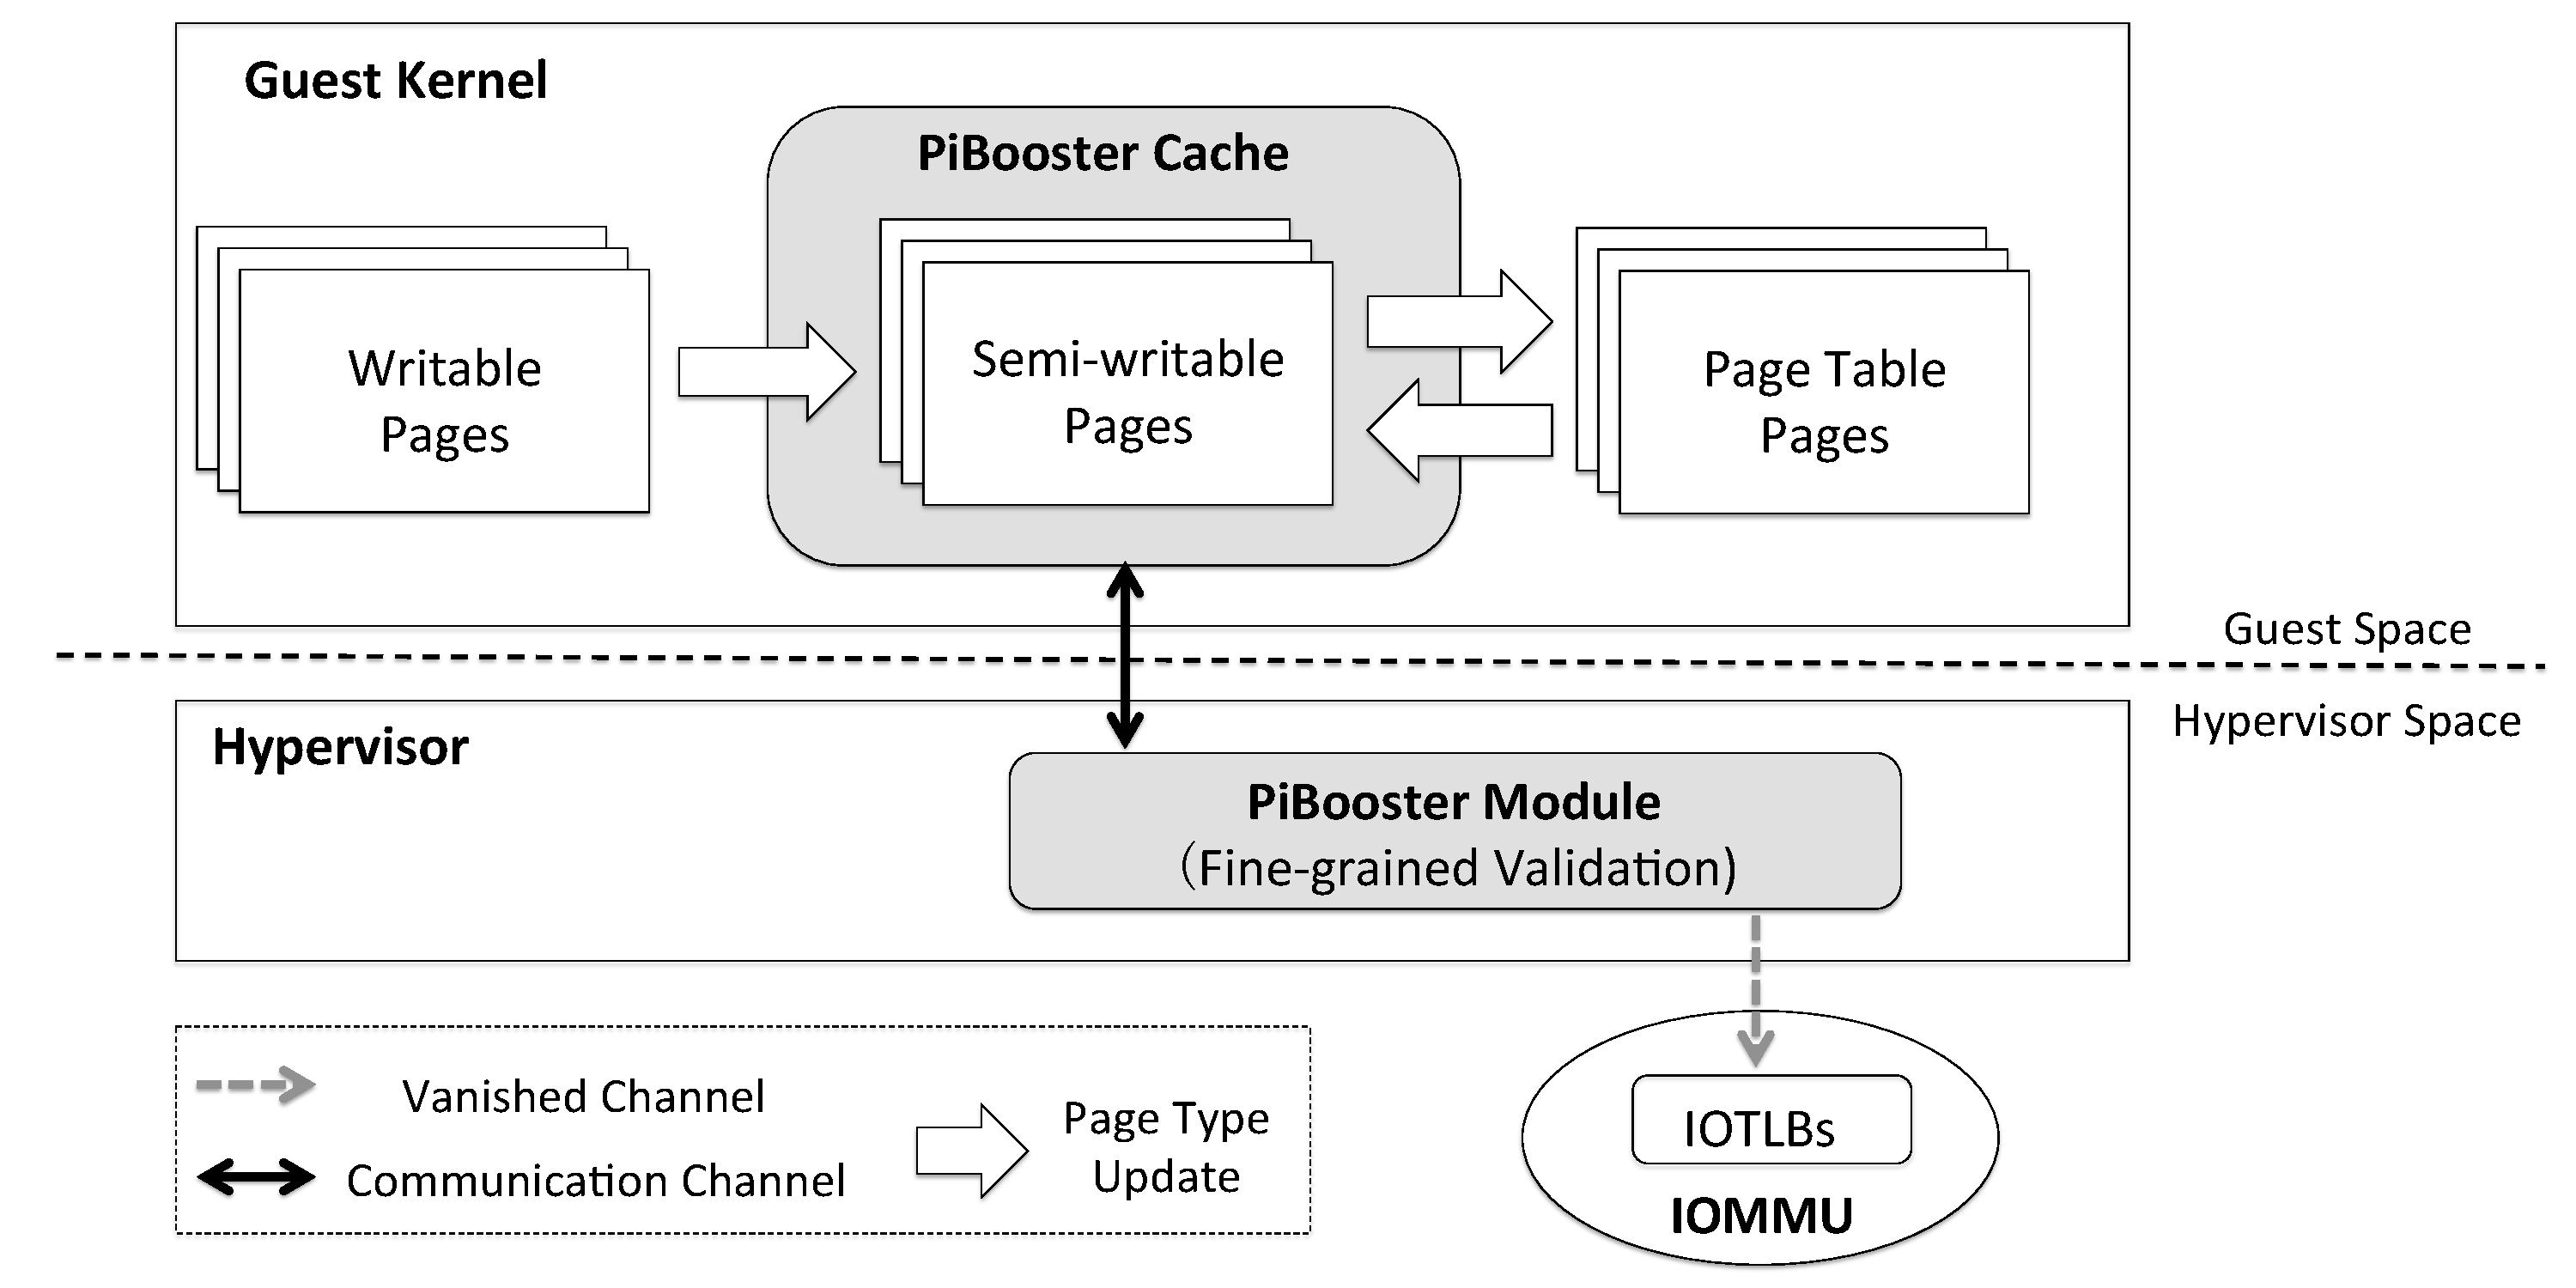
\includegraphics[width=0.8\textwidth]{image/overview/arch.pdf} \\
\caption{\name Architecture. The semi-writable pages are managed by the \name cache, and all page type updates are validated by the \name module.
Through the cooperation of \name cache and \name module, \name successfully shortens the execution paths of the guest page table (de)allocations and eliminates additional IOTLB flushes.}
\label{fig:arch}
\end{figure*}

\subsection{Design Requirements}\label{sec:req}
In the design of \name, we consider several requirements, which are summarized and listed as follows.
\begin{enumerate}
\item Unaltered system security. The new scheme should not sacrifice the system security to obtain performance benefits. No one likes to use a system with known design loopholes.
\item Compatible with legacy applications. The new scheme should limit the modifications on the guest kernel and the hypervisor, without any modifications on the existing applications.
\item Small modifications. The new scheme should minimize the development cost on the guest kernel and the hypervisor.
%\item Minimizing additional IOTLB flushes. The new scheme should minimize the number of IOTLB flushes, such as reducing the number to zero.
\end{enumerate}

\subsection{\name Architecture}
Figure~\ref{fig:arch} depicts the architecture of \name. It consists of a \cache in the guest kernel and a \name module in the hypervisor space.
%the mechanism of the \cache
The \cache allocates a number of semi-writable pages at the initial stage,  which are newly introduced by the fine-grained validation scheme (Section~\ref{sec:fine-grained}).
These semi-writable pages are maintained in a dedicated cache.
At runtime, the \cache attempts to satisfy all page table allocation and deallocation requests, shortening the execution path and saving the execution time.
There are many page type updates from/to the semi-writable pages.
The \cache mediates these updates and issues hypercalls to the hypervisor, asking it to perform the fine-gained security validations on the update requests (i.e., the communication channel).
Once the verified pages pass the validations, their page types will be updated accordingly.
%The guest kernel cannot bypass the security validation process, as the hypervisor is the only one to determine/update the page type.

The \module enforces the fine-grained validation scheme on the page table updates.
It performs (1) the page table validations that validate the page table contents as well as the type reference count, and (2) the DMA validations that ensure that the DMA requests cannot write the page-table pages and the semi-writable pages.
In the traditional validation scheme, the DMA validations always trigger additional IOTLB flushes due to the access permission updates between the writable pages and the page-table pages.
In the fine-grained validation scheme, both semi-writable pages and page-table pages are non-writable for DMA requests.
Thus, the hypervisor never needs to do the IOTLB flushes or IOMMU page table updates (i.e., vanished channel), which will benefit the I/O performance of the peripheral devices.
Moreover, it also saves the time of the whole security validation, further reducing the execution time of the page table allocations and deallocations.


\subsection{Fine-Grained Validation}\label{sec:fine-grained}
%To reduce the number of the IOTLB flushes, a possible approach is to let the hypervisor to manage the page table in its own space.
%In this way, there is no need for flushing IOTLB, but it will dramatically increase the size of the hypervisor, and consequently reduce the system security level.
%Another possible approach is to do the IOTLB flushing in a batch, meaning flushing multiple IOTLB entries all in one, instead of flushing them one after another.
%This approach is able to retain the system security, but it could not eliminate the IOTLB flushes, only reducing the number of IOTLB flushes in a certain level.
%In addition, this approach may result in security loopholes as the IOTLB entries are not synchronized with the corresponding IOMMU page table slots.
The fine-grained validation scheme aims to eliminate the additional IOTLB flushes and reduces the total time of the security validations.
Specifically, in the traditional security validation scheme, there are only two general page types: writable page and non-writable page,
and the type updates between them are required to do both page table validations and DMA validations.
The DMA validations not only increase the total validation time, but also introduce numerous additional IOTLB flushes.
%, which are likely to reduce the I/O performance of all related peripheral devices.
Moreover, the additional IOTLB flushes cannot be skipped, because it would provide a time gap for the adversary to attack the hypervisor by leveraging the stale IOTLB entries.
%1) bad impacts of original coarse-grained validation scheme 1) additional IOTLB flushes, and 2) long validation process

%2) How to do the fine-grained validation 1) semi-writable page 2) new page type updates 3) why save time and eliminate IOTLB flushes
To address this problem without sacrificing the system security, we introduce a new page type: \emph{semi-writable page}, which is writable for software but non-writable for DMA.
In addition, we enforce that the page type updates between the writable page and the page-table page must go through the semi-writable page first (as illustrated in Figure~\ref{fig:arch}).
As the semi-writable page and page-table page are already inaccessible to DMA, there is no need to do the DMA validations, meaning that the additional IOTLB flushes could be totally avoided.
As a consequence, the time of the whole security validation process is reduced, accelerating the speeds of page table allocations and deallocations.
%In order to facilitate the management of the semi-writable pages, we propose a cache, called \cache, in the guest kernel, and extend the existing page management data structure in the hypervisor space.
Similar to the management of the page-table pages, the hypervisor is only responsible for the final validation of the semi-writable page, leaving all other management operations for the \cache.
By doing this, we can keep the modifications as small as possible by reusing existing validation process and page-table management subsystem, and also retain the system security.


\subsection{\name Module}\label{sec:module}
The \module works in the hypervisor space, extended from the traditional coarse-gained validation module.
The first task of the \module is to add the support for the \emph{semi-writable page}.
Instead of adding a new data structure for marking the semi-writable pages, the \module chooses to reuse the existing one.
By doing so, the \module could reuse the existing interfaces.
In particular, we find that the page-type data structure could be extended by borrowing a bit from \emph{type reference count} for \emph{semi-writable page}.

The second task of the \module is to perform the fine-grained security validations for all page type update requests.
The main logic is to check page type first, and then determine to perform one validation or both of them.
Specifically, if the page type update occurs between writable page and semi-writable page, it will perform both page table and DMA validations.
However, if the page type update occurs between semi-writable page and page-table page, the \module only perform the page table validations, skipping the DMA validations.
Note that the page table validations are always necessary, as the semi-writable pages are writable for the guest OS, and the modifications from the untrusted guest OS could subvert the enforced security policies.

%For the DMA validations, they can be skipped, as both semi-writable page and page-table page are always non-writable for all DMA requests.
%The DMA requests are never able to subvert the integrity of the page table pages.
%This is why the additional IOTLB flushes are vanished.
%However, the page table validations are always necessary, as the semi-writable pages are writable for the guest OS, and the modifications from the untrusted guest OS could subvert the enforced policies.

The \module also exports a new hypercall interface for the \cache to facilitate their communications.
Through the new interface, the \cache could explicitly invoke the \module to perform security validations on specific page type updates.

\subsection{\name Cache}\label{sec:cache}
The basic idea behind the \cache is to have caches of semi-writable pages available for page table allocations and deallocations.
Without the page-oriented \cache, the kernel will spend much of its time allocating, initializing and freeing page-table pages.
The slab allocator that is similar to the \cache is not used in our settings, due to the following reasons.
%unaware of the page type updates
First, it is not aware of the page type or the security requirements, which would lead to unexpected crashes of the guest OS.
Adding such functionalities would introduce many internal checking operations that are necessary for other objects maintained by the slab allocator.
At least, those additional checking operations will lower the (de)allocation efficiency of other objects.
Second, the existing size-oriented management of the slab does not distinguish the page-table pages from other pages that have the same size, and the customization of this management mechanism would need lots of development costs, such as interface updates, internal data structure updates.
In addition, the related components that rely on the slab allocator may also be affected.
At last, adding the fine-grained validation mechanism only for one object (i.e., page-table page) will subvert the generality of the slab allocator.
Considering the above three reasons, we give up reusing the existing slab allocator and aim to build a dedicated one, maintained by \cache, serving the page table allocations and deallocations.

\subsubsection{\name Cache Initialization and Destruction}
The \cache is enabled in the system bootup phase by default.
By doing so, the page tables of all user processes are served by the \cache from the very beginning.
To increase the flexibility, it also allows dynamical activation at runtime through an exported interface.

In the initialization phase, the \cache allocates a bulk of pages from the existing system allocators, converts them into semi-writable pages, and maintains them in a dedicated cache list.
At runtime, the page table is always successfully deallocated by efficiently pushing deallocated pages into the \cache.
But the cases for the page table allocation is a little bit complex.
Normally, the \cache could serves all page table allocation requests using the cached pages.
However, in the worst cases, the cached pages may not be able to satisfy the allocation requests.
In such conditions, the \cache will have to re-invoke the system allocators to get new pages.
Fortunately, the reinvocations could be avoided by carefully setting the number of the initial pages.
In fact, the re-invocations rarely occur in a workflow stable system.
In our experiments, there are always several  semi-writable pages in the \cache ready for the page-table allocations after the \name is running for a few minutes.
All these cases are evaluated in Section~\ref{sec:eva}.

The \cache works in the whole life cycle of the guest by default, but the end user is able to explicitly disable it at any time through the exported interface.
Once the \cache receives the \emph{disable} command, it will release all resources, e.g., deallocating the cached pages assisted by the existing system allocators as well as the \module, and releasing the data structures that are used for managing the cached pages.
In addition, it will also issue a hypercall to inform the hypervisor, which will disable the fine-grained validation mechanism and switch it back to the traditional coarse-grained validation scheme.
%As the disable costs are quite high, we recommend that always keeping the \name running once it starts to work.

\subsubsection{Cache Shrinking}
When the memory management daemon (e.g., \emph{kswapd}) notices that the available memory is tight, it will explicitly call the exported interfaces of the \cache to free some cached pages.
%talk about the interface
There are two interfaces to shrink the cache pages. One is based on the page number. The memory management daemon can specify a number to ask the \cache to release.
The other one is based on the percentage. For instance, the kernel could ask the \cache to release 50\% cached pages.
%the size of the cache.
In fact, the number of semi-writable pages maintained in the \cache is not too high. In our experiments, it is always less than $180$, meaning that the size of the cache is less than $720KB$.

The \cache could also automatically shrink itself through a predefined threshold.
The threshold can be defined according to the page number or the proportion (i.e., the number of the cached semi-writable pages over the number of the page-table pages), or a combination of them.
%In the current prototype, the threshold is the combination of the page number and the percentage.






